% Appendix A

\chapter{Installation of OptiX} % Main appendix title

\label{AppendixA} % For referencing this appendix elsewhere, use \ref{AppendixA}

\lhead{Appendix A. \emph{Installation of OptiX}} % This is for the header on each page - perhaps a shortened title

\lstdefinestyle{DOS}
{
    backgroundcolor=\color{black},
    basicstyle=\scriptsize\color{white}\ttfamily
    numbers=none,
    numbersep=8pt,                   % how far the line-numbers are from the code
    numberstyle=\tiny\color{white}, % the style that is used for the line-numbers
    stepnumber=1                    % the step between two line-numbers. If it's 1, each line will be numbered
}
%----------------------------------------------------------------------------------------
\lstdefinestyle{C}
{
  morekeywords={export}
}
%----------------------------------------------------------------------------------------

This appendix will introduce how to install and verify the correct operation of the OptiX Ray Tracing Engine. Since OptiX is a CUDA-based framework, this installation is composed of 2 steps: Installation of CUDA Toolkit and installation of OptiX SDK. Note that OptiX is not listed in the \textit{Logithèque} of \textit{Calibre 7} (a Debian based distribution developed at EDF); a root account during installation is required.

%----------------------------------------------------------------------------------------

\section{Pre-installation Actions}
Some verifications must be taken before the entire process of installation:

%----------------------------------------------------------------------------------------

\subsection{Verify the System Has a CUDA-Capable GPU}
First of all, as a GPU framework developed by Nvidia, OptiX requires a CUDA-supported device. To verify if your GPU is CUDA-capable, open your \textit{Terminal} and enter:
\begin{lstlisting}[style=DOS][language=bash]
  $ lspci | grep -i nvidia
\end{lstlisting}
If the shown GPU can be found in the following list: \href{http://developer.nvidia.com/cuda-gpus}{http://developer.nvidia.com/cuda-gpus}, it's CUDA-capable. Otherwise, you should look for another GPU.

%----------------------------------------------------------------------------------------

\subsection{Verify GCC Compiler}
The gcc compiler is generally installed as part of the Linux distribution. Either it was installed or should be installed manually by yourself, make sure the installed gcc is the same version which was used to build your Linux kernel (\fref{fig:gcc}), or you will surely get errors during next step. Confirm your Linux kernel information:
\begin{lstlisting}[style=DOS][language=bash]
  $ cat /proc/version
\end{lstlisting}
Using the following command in order to verify the version of gcc installed on your system:
\begin{lstlisting}[style=DOS][language=bash]
  $ gcc -v
\end{lstlisting}

\begin{figure}[htbp]
	\centering
		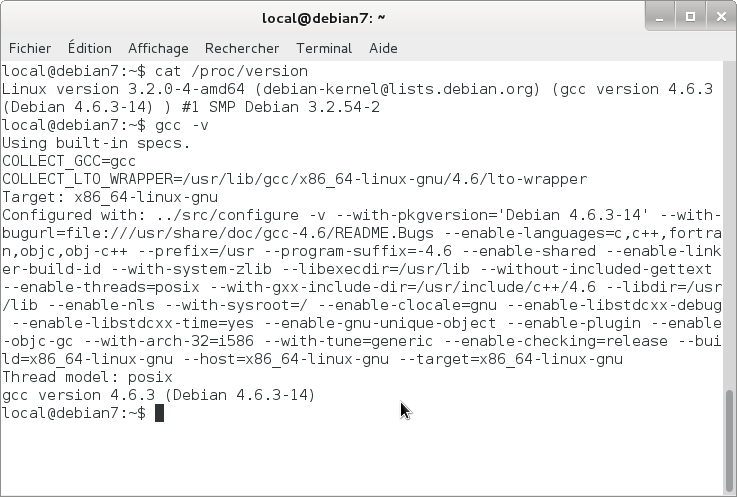
\includegraphics[width=13cm]{Figures/gcc.png}
	\caption{Verify the gcc compiler}
	\label{fig:gcc}
\end{figure}
After all these actions done, the installation can be continued to the next step.

%----------------------------------------------------------------------------------------

\section{Installation of CUDA Toolkit}
The NVIDIA CUDA Toolkit is available at \href{https://developer.nvidia.com/cuda-toolkit-archive}{https://developer.nvidia.com/cuda-toolkit-archive}. Choose and download the distribution-independent package ("RUN" package) for Ubuntu distribution, which corresponds to the \textit{Calibre} system. Notice that any architecture of CUDA is running based on a supported driver, for which an update is highly recommended. Although a driver update module is integrated in the CUDA installation package, it turns out not to be convenient for users: updates crash without any warning information. Therefore, one practical choice is to install respectively these two parts. Here we take a Nvidia Quadro FX 1800 as an example and install CUDA 5.5.22.
%----------------------------------------------------------------------------------------

\subsection{Installation of the NVIDIA Driver}
With the GPU information checked before, download the latest driver installation package: \href{http://www.nvidia.com/Download/index.aspx?}{http://www.nvidia.com/Download/index.aspx?}. In order to update a GPU driver, one should drop graphics interface on pressing \textit{Ctrl+Alt+F1} and stop \textit{X} server:
\begin{lstlisting}[style=DOS][language=bash]
  $ service gdm3 stop
\end{lstlisting}
To make the package executable, run the following:
\begin{lstlisting}[style=DOS][language=bash]
  $ sudo chmod x NVIDIA-Linux-x86_64-331.49.run
\end{lstlisting}
Install the NVIDIA driver on performing:
\begin{lstlisting}[style=DOS][language=bash]
  $ sudo ./NVIDIA-Linux-x86_64-331.49.run
  $ sudo reboot
\end{lstlisting}
Verify the driver has been successfully installed:
\begin{lstlisting}[style=DOS][language=bash]
  $ cat /proc/driver/nvidia/version
\end{lstlisting}

%----------------------------------------------------------------------------------------

\subsection{Installation of CUDA Toolkit}
Quit GUI on pressing \textit{Ctrl-Alt-F1} and begin installation by executing:
\begin{lstlisting}[style=DOS][language=bash]
  $ cat service gdm3 stop
  $ sudo chmod a+x cuda_5.5.22_linux_64.run
  $ sudo ./cuda_5.5.22_linux_64.run
\end{lstlisting}
Then the environment variables for our operating system need to be changed on editing the \textit{.bashrc} file:
\begin{lstlisting}[style=DOS][language=bash]
  $ gedit .bashrc
\end{lstlisting}
Add these two lines on the top of the current file and save:
\begin{lstlisting}[style=C]
    export PATH=/usr/local/cuda-5.5/bin:$PATH
    export LD_LIBRARY_PATH=/usr/local/cuda-5.5/lib64:$LD_LIBRARY_PATH
\end{lstlisting}


%----------------------------------------------------------------------------------------

\subsection{Verify the Installation of CUDA}
Before continuing, it is important to verify that the CUDA Toolkit can find and communicate correctly with the CUDA-capable hardware. To do this, you need to compile and run some sample programs.
Changing to the sample directory and compiling the examples:
\begin{lstlisting}[style=DOS][language=bash]
  $ cd ~/NVIDIA_CUDA-5.5_Samples 
  $ make
\end{lstlisting}
After compilation, run \textit{deviceQuery} and observe the result:
\begin{lstlisting}[style=DOS][language=bash]
  $ cd ~/NVIDIA_CUDA-5.5_Samples/bin/linux/release 
  $ ./deviceQuery
\end{lstlisting}
The output of this executable should look similar to the \fref{fig:cudatest}. Note that the important outcomes are that a device was found (the first highlighted line), that the device matches the one on your system, and that the test passed successfully (the second highlighted line).
\begin{figure}[htbp]
	\centering
		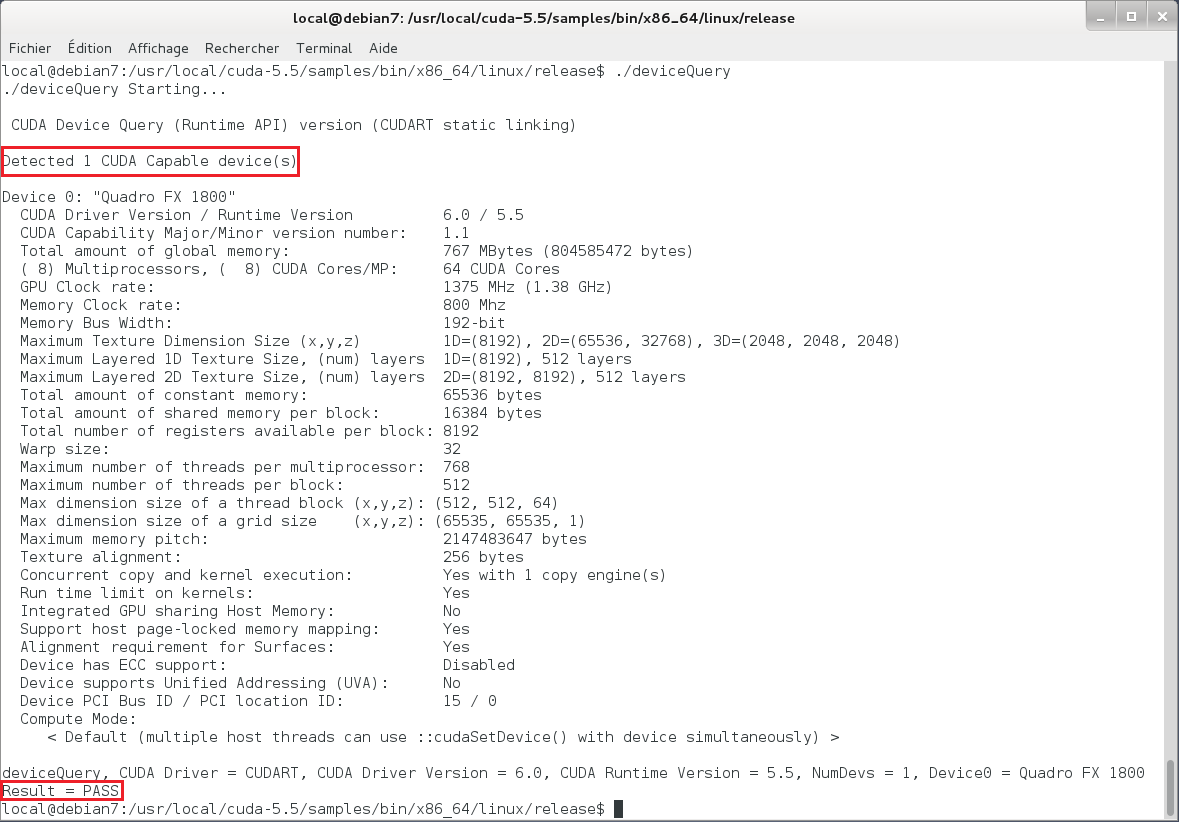
\includegraphics[width=13cm]{Figures/cudatest.png}
	\caption{CUDA test result}
	\label{fig:cudatest}
\end{figure}
%----------------------------------------------------------------------------------------

\section{Installation of OptiX SDK}
Unlike CUDA, there is no direct link to download an OptiX installation package. All developers need to create a special account: \href{https://www.surveymonkey.com/s/3D9FLR6}{https://www.surveymonkey.com/s/3D9FLR6}, two or three days later you will receive an email with your username and password inside. Then go to: \href{https://ftpservices.nvidia.com}{https://ftpservices.nvidia.com} and download corresponding installation package. Since the registration may take long, you can get a direct access with following coordinates:
\begin{itemize}
  \bf
  \item Username: OptiX-Beta-137
  \item Password: OptiX-Prime-Raytracing
\end{itemize}
To fully explore all features of OptiX, we choose to install the latest release at present: OptiX 3.5.1. Run the installation package:
\begin{lstlisting}[style=DOS][language=bash]
  $ sudo chmod a+x NVIDIA-OptiX-SDK-3.5.1-linux64.run
  $ sudo ./NVIDIA-OptiX-SDK-3.5.1-linux64.run
\end{lstlisting}
%----------------------------------------------------------------------------------------

\subsection{Post-installation Setup}
Establish links to OptiX library files:
\begin{lstlisting}[style=DOS][language=bash]
  $ sudo ln -s /home/local/NVIDIA-OptiX-SDK-3.5.1-PRO-linux64/lib64/liboptix.so.1 /usr/lib/liboptix.so.1
\end{lstlisting}
\begin{lstlisting}[style=DOS][language=bash]
  $ sudo ln -s /home/local/NVIDIA-OptiX-SDK-3.5.1-PRO-linux64/lib64/liboptixu.so.1 /usr/lib/liboptixu.so.1 
\end{lstlisting}
\begin{lstlisting}[style=DOS][language=bash]
  $ sudo ln -s /home/local/NVIDIA-OptiX-SDK-3.5.1-PRO-linux64/lib64/liboptix_prime.so.1 /usr/lib/liboptix_prime.so.1 
\end{lstlisting}

%----------------------------------------------------------------------------------------
